\begin{figure}[t]
    \centering
    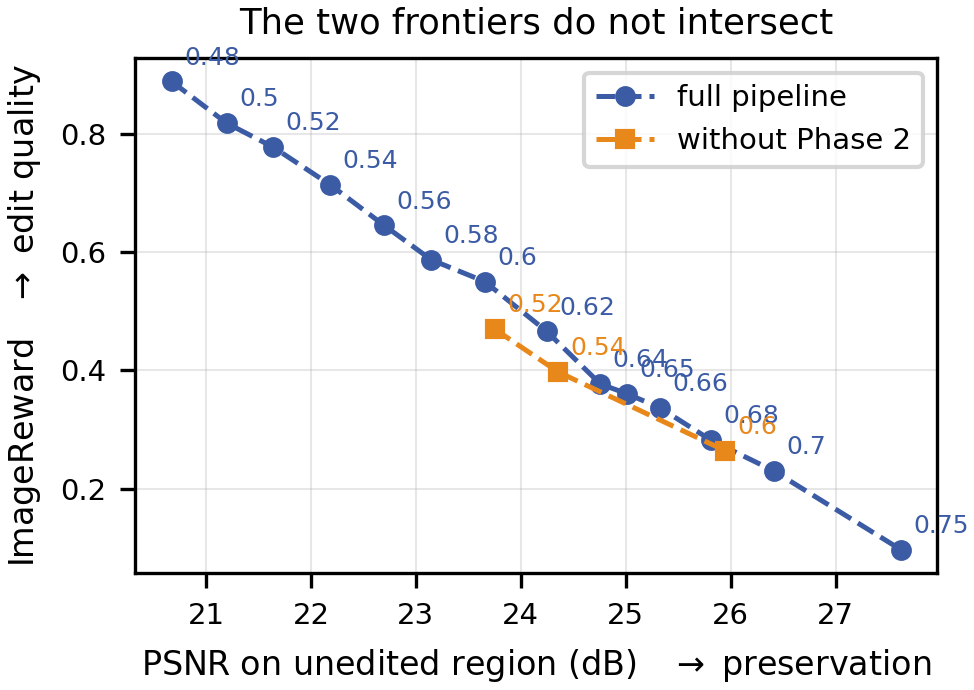
\includegraphics[width=\linewidth]{imgs/fig_beta_frontier.png}
    \caption{Ablating Phase~2 moves the whole frontier rather than the operating point along it. Labels give $h$. The ablated curve improves every preservation metric, but the two curves do not intersect in the overlapping range: at matched PSNR the full pipeline still leads by $\approx0.08$ ImageReward, and any point the ablated variant reaches is reached better by the full pipeline at a higher $h$.}
    \label{fig:beta_frontier}
\end{figure}
